\documentclass[11pt,a4paper]{article}
\usepackage[margin=0.9in]{geometry}
\usepackage[T1]{fontenc}
\usepackage[utf8]{inputenc}
\usepackage{graphicx}
\usepackage[hypertexnames=false]{hyperref}
\usepackage{enumitem}
\usepackage{float}
\usepackage{booktabs}

\title{Unsupervised Machine Learning\\arXiv Topic Clustering Report}
\author{Peter Dobosi}
\date{\today}

\begin{document}
\maketitle

\section*{Goal}

The goal of this homework is to solve a clustering-focused unsupervised
learning problem on recent arXiv papers from \texttt{cs.LG} and
\texttt{cs.CL}. I use paper titles and abstracts to discover broad research
topics, inspect how those topics vary over time, and demonstrate a small
content-based recommender.

The dominant assignment component is clustering. The recommender is included
as a secondary use of the same document representation.

\section*{Course Alignment}

The implementation follows the structure and tools covered in the course
materials:

\begin{itemize}[leftmargin=*,itemsep=2pt]
    \item \textbf{Document similarity}: cosine similarity is used for text
    vectors because vector direction is more informative than raw vector
    length for abstracts.
    \item \textbf{Dimensionality reduction}: TF-IDF is compressed with
    truncated SVD into latent semantic analysis (LSA) features, and PCA is
    used for a two-dimensional visualisation.
    \item \textbf{Clustering}: KMeans, Ward agglomerative clustering, and
    HDBSCAN are compared.
    \item \textbf{Internal validation}: Silhouette, Davies-Bouldin, and
    Calinski-Harabasz scores are reported for the clustering comparison.
    \item \textbf{Recommendation}: the final helper is content-based rather
    than collaborative because no user-paper rating matrix is available.
\end{itemize}

\section*{Method}

\begin{enumerate}[leftmargin=*,itemsep=2pt]
    \item \textbf{Data acquisition}: I fetched a balanced monthly sample of
    arXiv papers from the previous 12 months. The final cached corpus contains
    1,848 papers, with 154 papers per month from May 2025 through April 2026.

    \item \textbf{Text cleaning and representation}: Titles and abstracts are
    concatenated, URL-like tokens are removed, and a TF-IDF matrix is fitted
    with unigrams and bigrams. I also compute a 100-dimensional dense LSA
    representation with truncated SVD.

    \item \textbf{Clustering comparison}: KMeans, Ward agglomerative
    clustering, and HDBSCAN are run on the dense LSA representation. The same
    algorithms are also evaluated on sparse TF-IDF, with dense conversion only
    where required by the implementation.

    \item \textbf{Topic interpretation}: The best practical clustering result
    is interpreted with high-weight TF-IDF terms and representative papers
    closest to each KMeans centroid.

    \item \textbf{Visualisation and recommendation}: I generate a PCA scatter
    plot, a topic-size bar chart, a smoothed topic timeline, and a
    content-based recommender using cosine similarity in LSA space.
\end{enumerate}

\subsection*{Implementation Note}

The initial plan included transformer-based scientific embeddings and a
BERTopic layer. During execution, that path pulled a very large PyTorch/CUDA
dependency chain and the install did not complete in a useful time window.
Because the assignment is time-sensitive and clustering is the dominant
requirement, I changed to a lighter and fully reproducible TF-IDF plus LSA
pipeline. This still covers the planned clustering comparison, internal
metrics, topic interpretation, visualisation, and recommender components.

\section*{Results}

\begin{table}[H]
\centering\small
\begin{tabular}{llrrrrr}
\toprule
\textbf{Representation} & \textbf{Method} & \textbf{Clusters} & \textbf{Outliers} & \textbf{Sil.} & \textbf{DB} & \textbf{CH} \\
\midrule
LSA & KMeans & 14 & 0.0\% & 0.075 & 4.09 & 23.48 \\
LSA & Ward & 14 & 0.0\% & 0.029 & 4.50 & 17.77 \\
LSA & HDBSCAN & 4 & 91.2\% & 0.257 & 2.33 & 17.01 \\
TF-IDF & KMeans & 16 & 0.0\% & 0.007 & 10.27 & 3.32 \\
TF-IDF & Ward & 16 & 0.0\% & 0.002 & 9.31 & 3.19 \\
TF-IDF & HDBSCAN & 0 & 100.0\% & -- & -- & -- \\
\bottomrule
\end{tabular}
\caption{Internal clustering metrics. HDBSCAN scores are computed on
non-outlier papers only, so its high LSA silhouette is not directly comparable
to the full-coverage KMeans result.}
\label{tab:clustering}
\end{table}

KMeans on cleaned LSA is the best practical configuration. HDBSCAN identifies
small dense groups, but it marks most papers as outliers. Direct TF-IDF
clustering is much weaker by all internal metrics.

\begin{table}[H]
\centering\small
\begin{tabular}{rlr}
\toprule
\textbf{Topic} & \textbf{Keyword label} & \textbf{Papers} \\
\midrule
5 & llms, language, language models, llm & 254 \\
3 & training, model, models, data & 254 \\
0 & data, learning, optimization, gradient & 223 \\
13 & machine, machine learning, learning, data & 173 \\
4 & neural, networks, neural networks, graph & 163 \\
1 & agent, agents, multi, multi agent & 135 \\
8 & diffusion, generative, generation, diffusion models & 103 \\
10 & reasoning, llms, cot, models & 94 \\
\bottomrule
\end{tabular}
\caption{Largest KMeans-LSA topics after cleaning URL-like tokens.}
\label{tab:topics}
\end{table}

\begin{figure}[H]
    \centering
    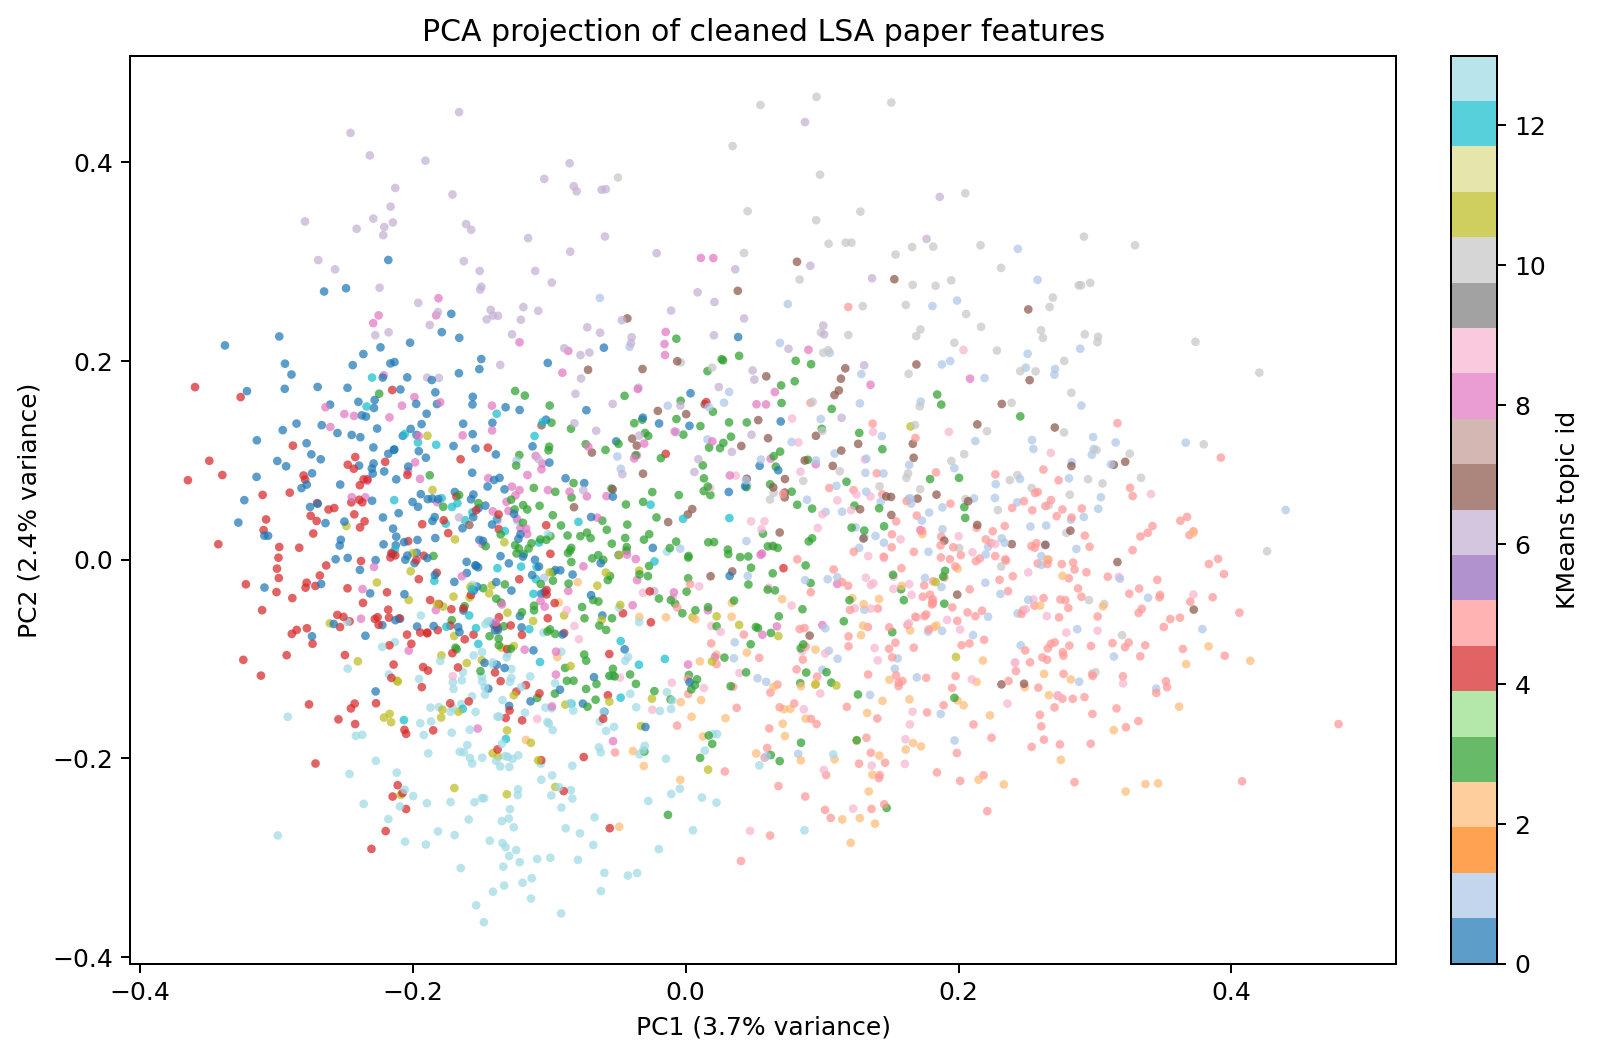
\includegraphics[width=0.95\textwidth]{output/pca_topic_scatter.png}
    \caption{PCA projection of the cleaned LSA features, coloured by KMeans
    topic id. The overlap supports the interpretation that arXiv topics are
    continuous and partially mixed rather than sharply separated.}
    \label{fig:pca}
\end{figure}

\begin{figure}[H]
    \centering
    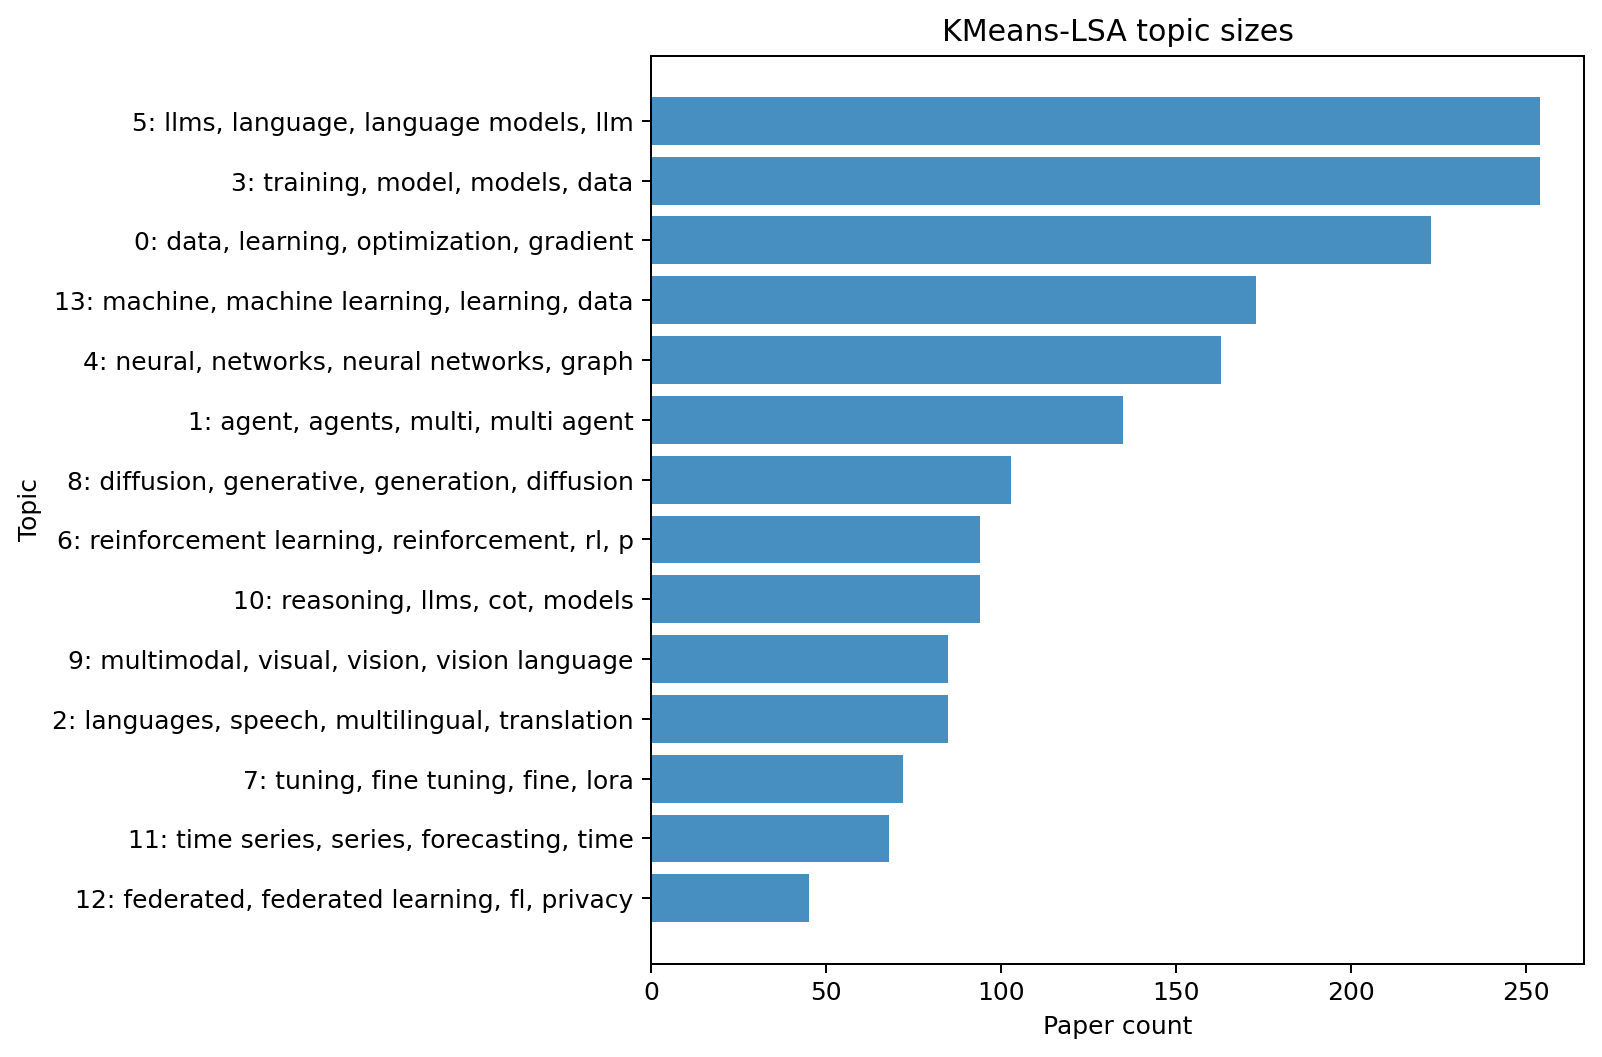
\includegraphics[width=0.95\textwidth]{output/topic_sizes.png}
    \caption{Topic sizes for the selected KMeans-LSA model.}
    \label{fig:sizes}
\end{figure}

\begin{figure}[H]
    \centering
    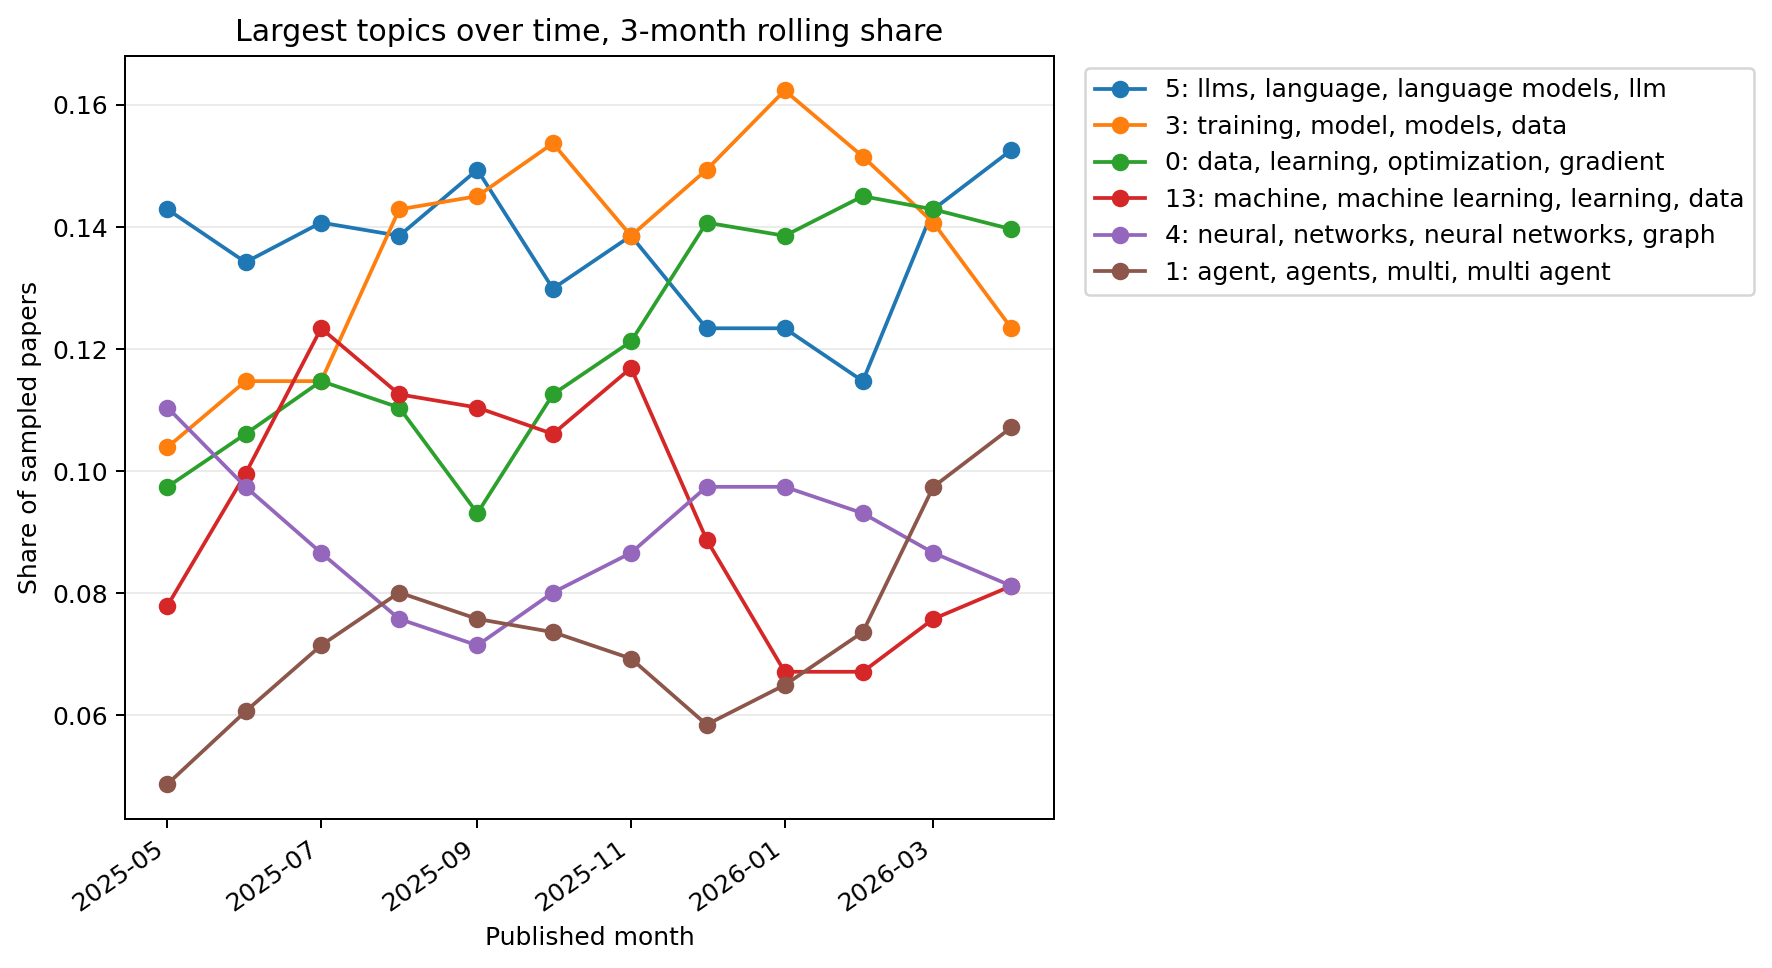
\includegraphics[width=0.95\textwidth]{output/topic_timeline_rolling.png}
    \caption{Three-month rolling topic share for the largest topics. The plot
    is exploratory because each month contains a fixed sample of about 154
    papers.}
    \label{fig:timeline}
\end{figure}

\section*{Discussion}

The KMeans elbow curve is fairly gradual, which is expected for research
abstracts. Papers often combine methods and application areas, so the corpus
does not form perfectly separated geometric clusters. I therefore treat the
selected number of topics as a useful granularity, not as a unique natural
truth.

The strongest result is the representation comparison: raw sparse TF-IDF is
not enough for coherent clustering, while cleaned LSA gives a much more useful
topic structure. The URL-token cleaning step also mattered: without it, one
cluster was dominated by repository-link tokens rather than scientific
content.

The recommender demonstrates a second use of the learned representation. Given
a query abstract, the system transforms it with the fitted TF-IDF and LSA
models, then returns papers with the highest cosine similarity. This is a
reasonable content-based alternative when collaborative filtering data is not
available.

\section*{Conclusion}

The final notebook completes a clustering-dominant unsupervised learning
pipeline with data acquisition, representation learning, algorithm comparison,
topic interpretation, visualisation, and content-based recommendation. The
main practical conclusion is that cleaned TF-IDF compressed with LSA and
clustered by KMeans is a simple, reproducible baseline for exploring recent
arXiv topics under tight runtime constraints.

\end{document}
